\documentclass[11pt]{beamer}  %% versione proiettore
%%\documentclass[11pt,handout]{beamer} %% versione stampa
\usepackage{lucidiJb-2ed}

\usepackage{relsize}

\mode<article>
{
  \usepackage{fullpage}
  \usepackage{hyperref}
}

\mode<presentation>
{
  \setbeamertemplate{background canvas}[vertical shading][bottom=red!10,top=blue!10]
  \usetheme{Ethereum}
  \usefonttheme[onlysmall]{structurebold}
}

\subtitle{Learning Ethereum}
\title{Smart Contracts}
\institute{Universit\`a di Verona, Italy}
\date{January 2020}

\setbeamercovered{invisible}

\def\codesize{\smaller}
\def\<#1>{\codeid{#1}}
\newcommand{\codeid}[1]{\ifmmode{\mbox{\codesize\ttfamily{#1}}}\else{\codesize\ttfamily #1}\fi}

\begin{document}

\begin{frame}
  \titlepage
\end{frame}

\begin{frame}\frametitle{A simple Ponzi scheme}

  \begin{center}
    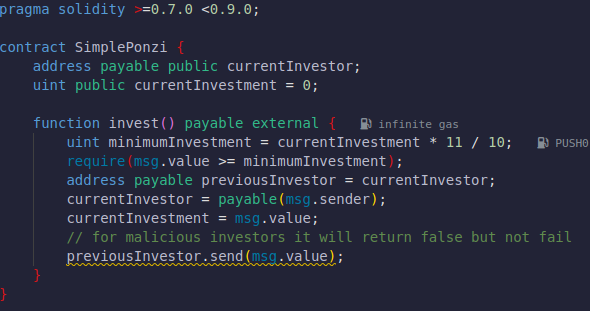
\includegraphics[width=\textwidth,clip=false]{pictures/simple-ponzi.png}
  \end{center}

  \bigskip

  The first investment will be burned to the address \<0x0>.
  
\end{frame}

\begin{frame}\frametitle{Exercise}
  \begin{enumerate}
  \item create an account with MetaMask
  \item charge it from the Ropsten faucet with 1 ETH
  \item write the \<SimplePonzi.sol> contract in Remix
  \item compile the contract in Remix
  \item deploy the contract in Ropsten with Remix
  \item connect to the contract in Ropsten by somebody else
  \item start calling the fallback function with increasing value
    (with Remix of with MetaMask; for the latter, remember to increase
    to gas limit for sending ETH)
  \end{enumerate}

  \bigskip
  You can check the current investment and investor from Remix.

\end{frame}

\begin{frame}\frametitle{A gradual Ponzi scheme}

  \begin{center}
    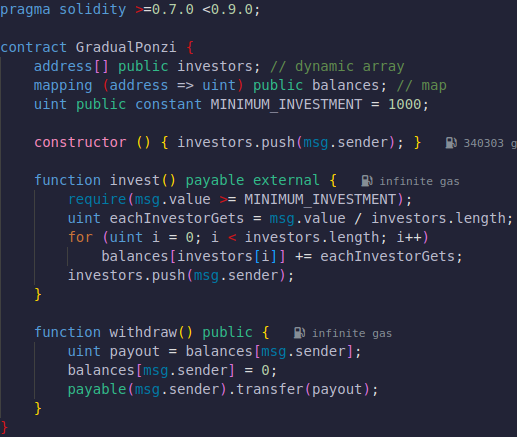
\includegraphics[scale=0.4,clip=false]{pictures/gradual-ponzi.png}
  \end{center}

\end{frame}

\begin{frame}\frametitle{A simple lottery (1)}

  \begin{center}
    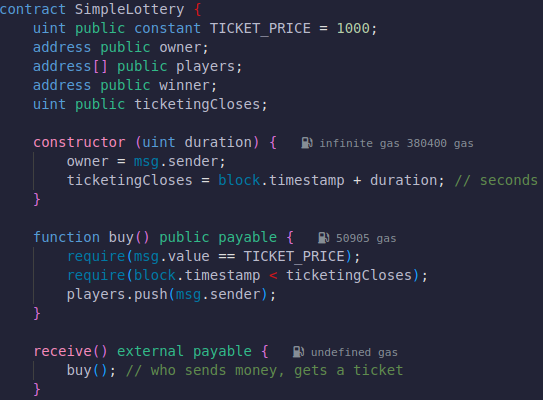
\includegraphics[scale=0.4,clip=false]{pictures/simple-lottery-1.png}
  \end{center}

\end{frame}

\begin{frame}\frametitle{A simple lottery (2)}

  \begin{center}
    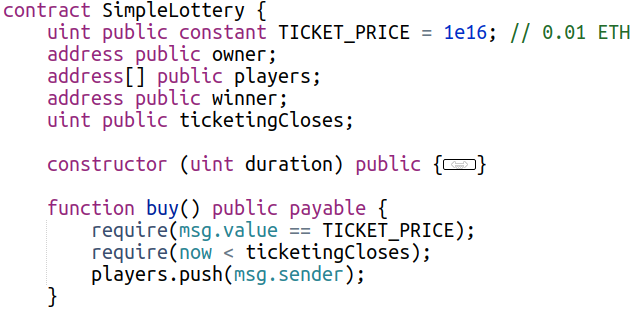
\includegraphics[scale=0.4,clip=false]{pictures/simple-lottery-2.png}
  \end{center}

\end{frame}

\begin{frame}\frametitle{A simple lottery (3)}

  \begin{center}
    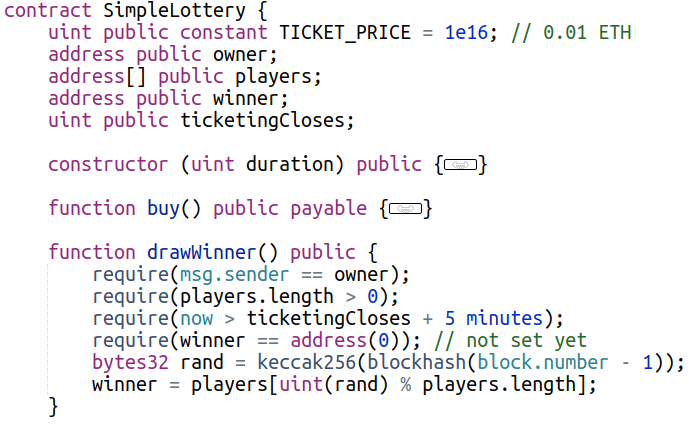
\includegraphics[scale=0.4,clip=false]{pictures/simple-lottery-3.png}
  \end{center}

\end{frame}

\begin{frame}\frametitle{A simple lottery (4)}

  \begin{center}
    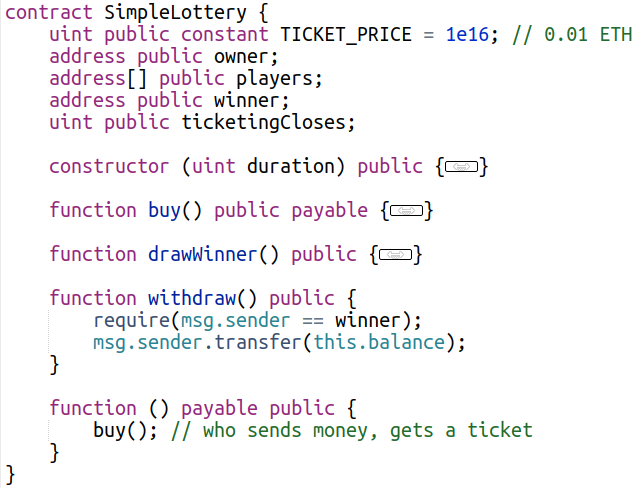
\includegraphics[scale=0.4,clip=false]{pictures/simple-lottery-4.png}
  \end{center}

\end{frame}

\begin{frame}\frametitle{Exercise}
  \begin{enumerate}
  \item create an account with MetaMask
  \item charge it from the Ropsten faucet with 1 ETH
  \item write the \<SimpleLottery.sol> contract in Remix
  \item compile the contract in Remix
  \item deploy the contract in Ropsten with Remix, with 3 minutes for buying tickets
  \item connect to the contract in Ropsten by somebody else
  \item buy some tickets before the 3 minutes expire
    (with Remix of with MetaMask; for the latter, remember to increase
    to gas limit for sending ETH)
  \item the owner of the lottery contract draws the winner
  \item try to withdraw your price (if any!)
  \end{enumerate}

  \bigskip
  You can check the winner from Remix.

\end{frame}

\end{document}
